\part{Savoir-faire et savoir-être: la mise en valeur de soi et de son travail dans les annonces d’emploi}



\chapter{Au cœur des annonces, la description des compétences domestiques}

Le format de l'annonce présente plusieurs difficultés pour quiconque cherche une place de domestique: elle doit être courte, impersonnelle, répondre à une mise en forme précise qui laisse peu de place à la différenciation ou à la créativité. Mais cette "expression de soi hautement contrainte\footcites{kramplPresseAnnoncesParisienne2020}" n'empêche pas les demandeurs et demandeuses de se présenter sous leur meilleur jour: la brièveté des publications permet malgré tout de se mettre en valeur et de taire ce qui, selon des normes de genre, d'âge ou de classe, éloigne du canon domestique. Cette mise en valeur passe notamment par la description de compétences ou de qualités physiques et morales. Dans cette partie, je considère donc l'annonce comme une forme de "publicité de soi", qui justifie la place des demandes d'emploi dans l'économie générale du journal d'annonces, et les rapproche d'autres types de textes publiés par les \textit{Affiches} (publicités commerciales, annonces immobilières, ...). Ainsi, dans le journal d'annonces, "l’emploi se trouve (...) d’office placé dans une logique de consommation, qui l’apparente, sinon l’assimile à un bien à échanger\footcites{kramplAdresserClercHuissier2017}". 

À travers l'étude de ce qui représente le corps de l'annonce, de ses éléments de langage les plus courants mais également des potentielles tentatives de distinction, il s'agit donc d'interroger ce qui constitue la "bonne" domesticité aux yeux des demandeurs et donc, par extension, des employeurs potentiels. 


\section{Méthode}

Parmi les différentes composantes de l'annonce, un élément, déjà signalé par l'historiographie, apparaît central: il s'agit des compétences avancées par les demandeurs et demandeuses, qu'Ulrike Krampl désigne sous le terme de "talents". Pour extraire ces informations, plusieurs méthodes ont été envisagées.

La première, la plus simple, consistait encore une fois en l'élaboration d'expressions régulières. Une lecture proche des annonces a en effet permis d'observer que, pour une part non négligeable du corpus, les compétences se situent toujours au même endroit : entre les mots "sachant" (ou "sait") et "désire" (ou "désireroit"). Les annonces qui répondent à ce critère formel très spécifique ressemblent alors à "Une jeune fille de 18 ans, sachant coudre et repasser, désire une PLACE de domestique...". Ainsi, l'expression régulière \fbox{\b(?:sachant|sait)\b (.*?) de?é?sir} trouve une correspondance dans 922 annonces. Les compétences ainsi extraites permettent de réaliser le nuage de mots suivants, déjà parlant quant à la surreprésentation (et donc la valorisation?) de certaines activités et savoir-faire domestiques (la cuisine, la couture, mais également le fait de savoir lire et écrire):

\begin{figure}[h]
	\centering
	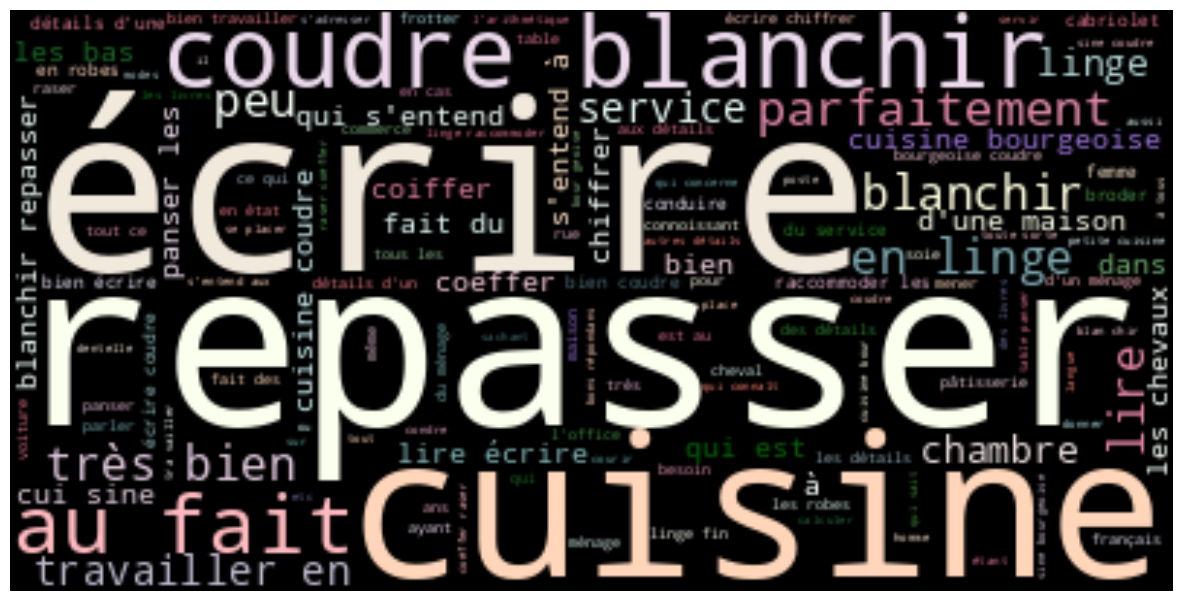
\includegraphics[width=12cm]{wordcloud_comp_regex.png}
	\caption{Nuage de mots des compétences extraites grâce aux expressions régulières}
\end{figure}

Si cette première méthode permet d'extraire les compétences avec une grande précision, elle n'est valable que pour une minorité des annonces (un cinquième du corpus). Pour les annonces ne répondant pas au modèle "...sachant [compétence], désire...", j'ai employé la librairie Spacy et sa fonction de \textit{span categorization}. Cette fonction permet, à la façon de la reconnaissance d'entités nommées (\textit{Named Entity Recognition}, ou NER), de repérer et de classer certaines parties d'un texte selon des catégories pré-définies par l'utilisateur. Néanmoins, contrairement au NER, la classification de \textit{spans} peut concerner n'importe quelle partie du texte, indépendamment de sa longueur, de sa classe ou de sa fonction grammaticale. Elle est donc plus à même de traiter des phrases ou des fragments de phrases, y compris lorsqu'ils se chevauchent. Dans notre cas, où les compétences sont signalées soit par leur place dans la structure de l'annonce, soit par certaines répétitions, cette méthode parait la plus prometteuse parmi celles proposées par Spacy.  Plus important encore ici, cette fonction est entraînable; il a donc été possible de développer un modèle propre au corpus d'annonces et à ses problématiques, sur la base d'annotations préalables. 



\newpage

\global\mdfdefinestyle{mystyle}{%
	linecolor=white,linewidth=3pt,%
	leftmargin=2cm,rightmargin=2cm
}

\begin{mdframed}[style=mystyle,frametitle={L'annotation du corpus}, backgroundcolor=LavenderBlush1] %
	
	
	Pour produire les données d'entraînement, j'ai utilisé Prodigy, un outil d'annotation disposant d'une interface en ligne et développé par l'équipe à l'origine de la librairie spacy. Pour annoter des \textit{spans}, il permet de sélectionner le texte à annoter (y compris sous forme de \textit{dataframe}), de choisir les catégories voulues (ici, compétences mais également emploi, qualités, adresse) puis de "surligner" les mots ou ensembles de mots correspondant à chaque catégorie. 	Une fois l'annotation terminée, Prodigy permet ensuite d'exporter directement les annotations au bon format et de générer automatiquement un fichier de configuration spacy. 
		
	\bigskip
	
	\centering
	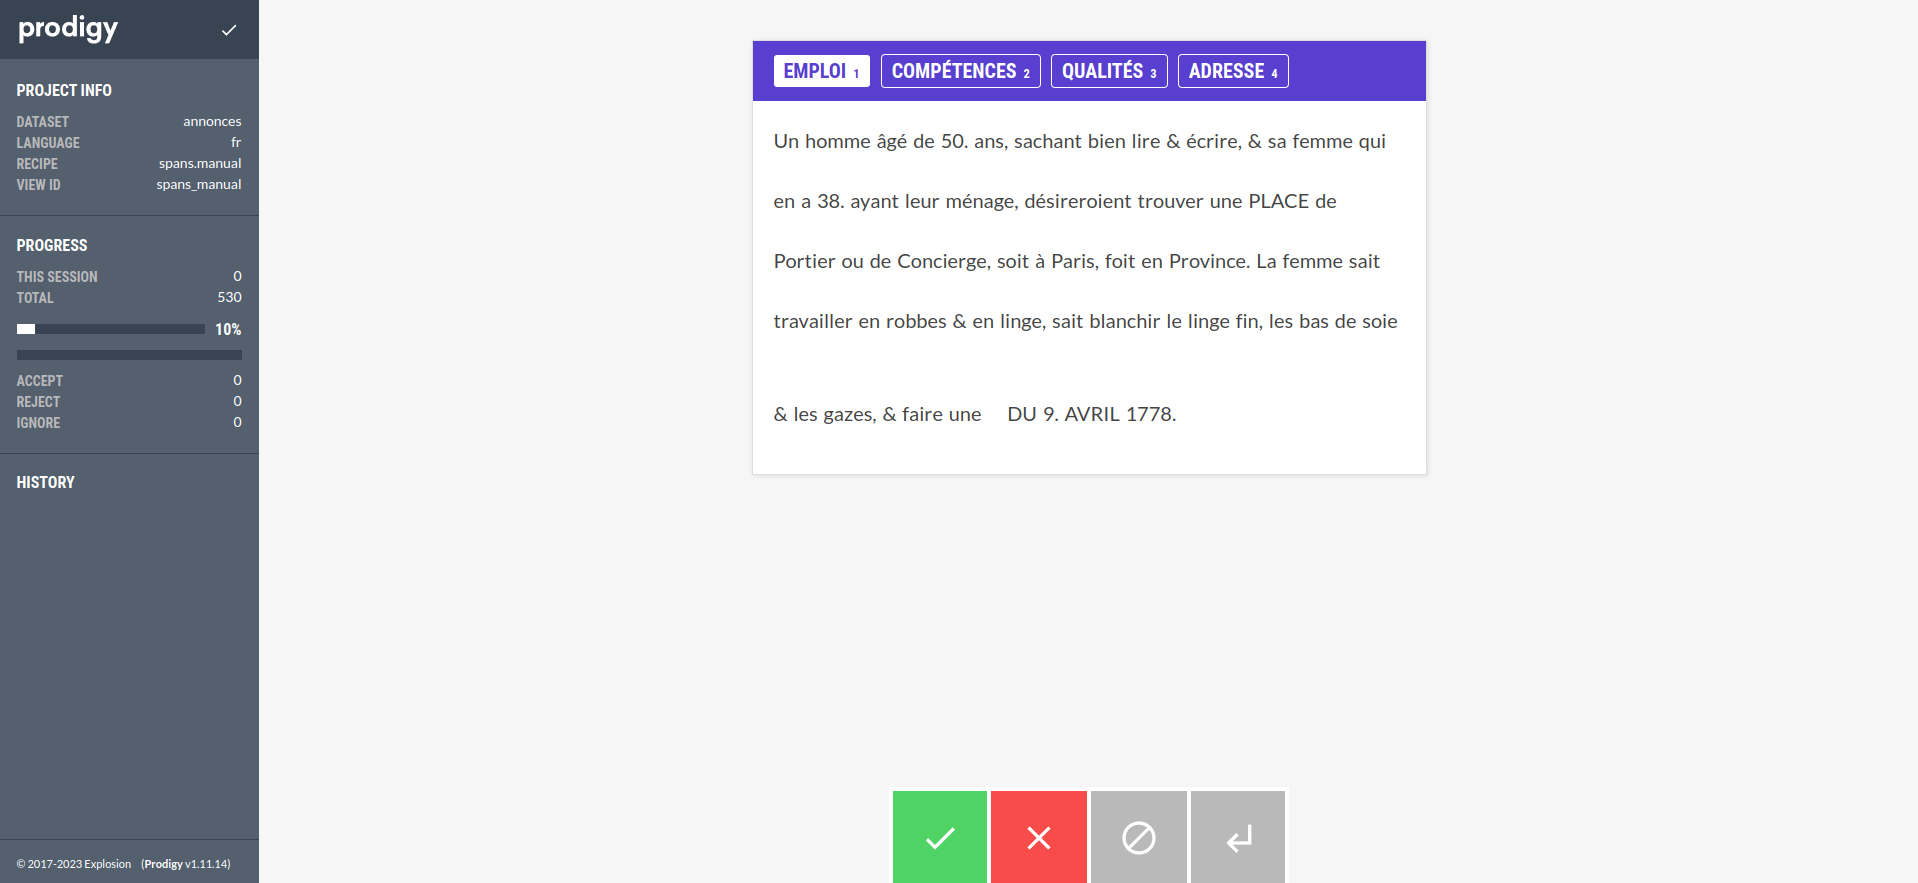
\includegraphics[width=10cm]{exemple_prodigy_1.png}
	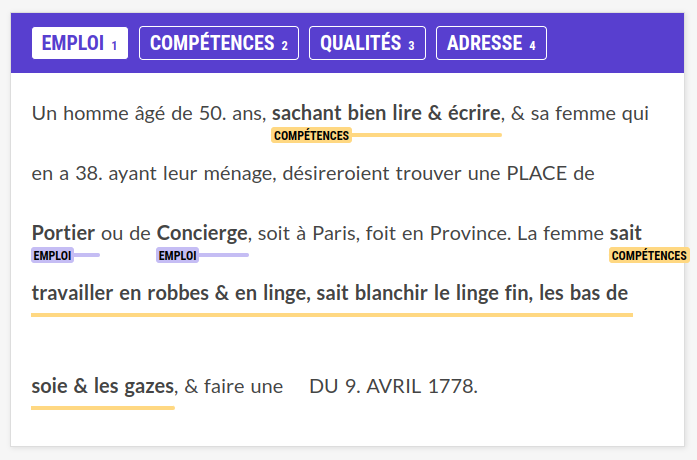
\includegraphics[width=10cm]{exemple_prodigy_2.png}
	\captionof{figure}{Exemples de l'interface Prodigy}
		
	\bigskip

		
\end{mdframed}

\bigskip

Afin de déterminer le nombre d'annonces à annoter, j'ai graduellement entraîné plusieurs modèles spacy, au fur et à mesure de l'annotation, et observé l'évolution des scores de performances du modèle en fonction du nombre d'annotation. Si les scores augmentent fortement entre la première et la 300ème annotation, ils commencent ensuite à stagner: un modèle entraîné sur la base de 300, 400 ou 500 annotations produira sensiblement les mêmes F1scores, autour de 0.6. Néanmoins, la précision (c'est-à-dire l'exactitude ou la pertinence des mots extraits et catégorisés par le modèle) est bien meilleure que le rappel (c'est-à-dire l'exhaustivité du modèle): tandis que la première se situe autour de 0.75, le second peine à dépasser 0.5. Cela signifie que le modèle, s'il parvient à bien extraire certaines compétences sans produire trop de faux positifs, n'est pas complet: il laisse de côté beaucoup d'éléments pertinents. Les compétences extraites seront donc dans leur ensemble bien des compétences, mais ne seront peut-être pas complètement représentatives; cette limite du modèle est évidemment à prendre en compte dans l'analyse.

\begin{figure}[ht]
	\centering
	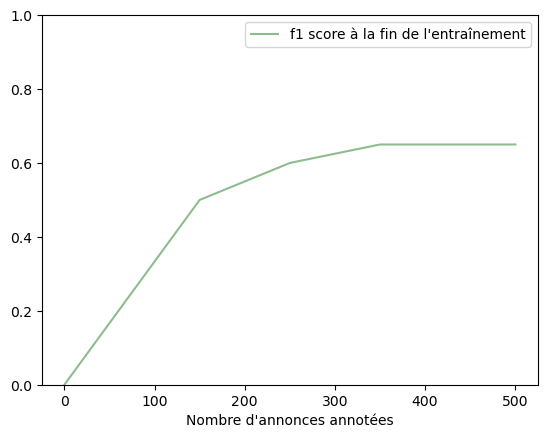
\includegraphics[width=12cm]{scores_span_cat.png}
	\caption{Évolution des scores de performance du modèle de catégorisation en fonction des annotations}
\end{figure}

\begin{figure}[ht]
	\centering
	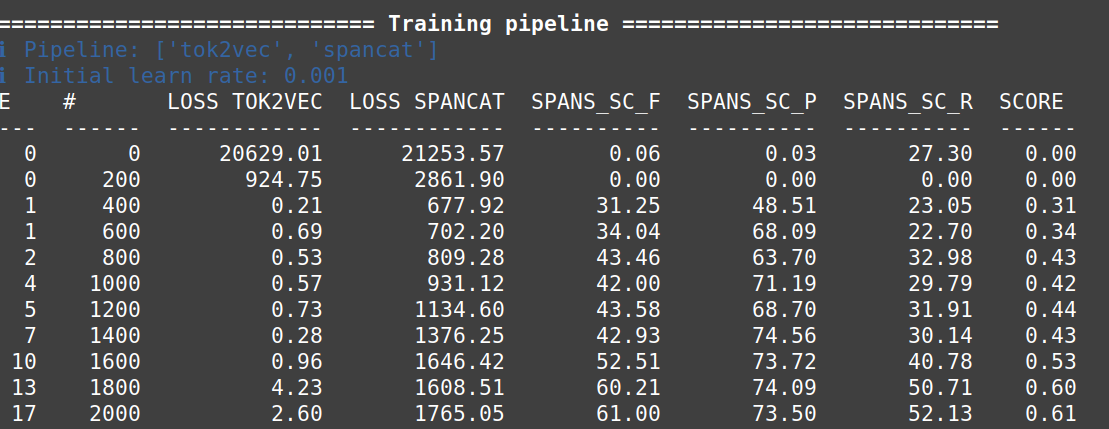
\includegraphics[width=12cm]{scores_entrainement_spacy.png}
	\caption{Évolution des scores de performance au cours de l'entraînement final}
\end{figure}

Une fois le modèle de \textit{span categorization} entraîné, une fonction a permis d'extraire les \textit{spans} catégorisés comme étant des compétences, puis d'ajouter une colonne dédiée au \textit{dataframe}. Au final, le modèle entraîné sur la base de 530 annotations permet ainsi de reconnaître 1701 annonces contenant des compétences.

\section{Lire, écrire et bien cuisiner: l'importance des verbes pour décrire des talents majoritairement manuels}

Un premier constat qui peut être fait sur la description des compétences dans les annonces est celui de l'uniformité formelle de celle-ci.  Les "talents" évoqués prennent la grande majorité du temps la forme de verbes ou d'expressions verbales ("repasser le linge", "faire une cuisine bourgeoise"). Cette caractéristique, en plus de montrer l'homogénéité éditoriale des \textit{Affiches}, fait écho à plusieurs travaux historiques, qui ont déjà montré l'importance du verbe dans la représentation et la description du travail à l'époque moderne, où l'activité des individus (notamment des femmes) est souvent plurielle et l'usage de noms de métiers encore rare. C'est notamment le cas du projet \textit{Gender and Work}, qui se base sur une méthode lexicale "orientée verbe" pour extraire automatiquement\footcites{petterssonParsingIdentificationVerb2012} les activités de sources modernes suédoises diverses (archives judiciaires, livres de compte, lettres, journaux...). Le projet s'est lui-même inspiré des travaux de Sheilagh C. Ogilvie sur l'histoire du travail des femmes en Allemagne\footcites{ogilvieBitterLivingWomen2003}. 

\begin{figure}[h]
	\centering
	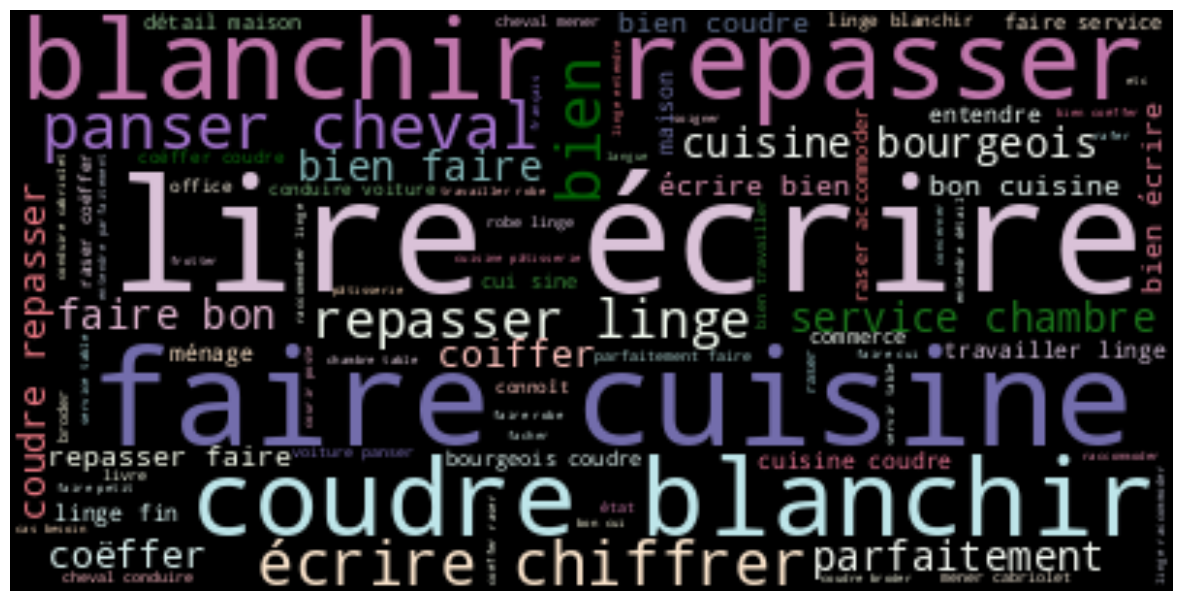
\includegraphics[width=10cm]{wordcloud_comp_spacy.png}
	\caption{Nuage de mots des compétences extraites grâce au modèle de \textit{span categorization}}
\end{figure}

Ces observations semblent se vérifier sur le corpus de petites annonces: sur 23156 tokens considérés par notre modèle comme des compétences, 5507 sont des verbes, soit plus d'un sur cinq. Sur 1701 annonces concernées, 1648 contiennent au moins un verbe de compétence; 991 en contiennent au moins trois.
De plus, l'analyse des mots les plus fréquents du corpus montre une grande uniformité des verbes employés, et donc des compétences mises en avant. L'écriture, notamment, est très valorisée: elle est présente dans près de la moitié des annonces, signe de l'alphabétisation croissante au XVIIIè siècle, mais aussi de l'avantage que cette capacité procure dans la recherche d'emploi réelle ou telle qu'elle est imaginée par les domestique. En dehors de l'écriture, de la lecture et, à une échelle moindre, du calcul, les compétences les plus réitérées sont surtout manuelles: coudre, repasser, coiffer, raser sont des aptitudes associées à une domesticité de service, aux tâches multiples dans la maison et plutôt peu qualifiée. Mais ces éléments à première vue très descriptifs sont parfois agrémentés d'adverbes ou d'adjectifs à valeur méliorative: près de la moitié des annonces contiennent au moins un adverbe, la plupart étant "bien" (492 occurrences) et "parfaitement" (179).
Certaines expressions ou ensembles de talents sont également très fréquentes, ce qui peut être observé à partir des bigrammes et trigrammes de mots: dans près d'un cas sur quatre, le mot "cuisine" fait partie de l'expression "faire une cuisine bourgeoise" (96 occurrences sur 416). Le diptyque "lire et écrire" est également très fréquent: 367 annonces mentionnent les deux compétences, 7 ne mentionnent que savoir lire et 273 mentionnent uniquement l'écriture. De même, les compétences liées au soin du linge vont souvent par paire, voire par trio: 117 annonces n'évoquent que la couture, 106 le fait de savoir "coudre et blanchir", 161 la capacité de "coudre, blanchir et repasser". 


\begin{table}[ht]
		\centering
			\begin{tabular}{lc}
			\hline
			\textbf{Mot} & \textbf{Occurrences} \\ \hline
			écrire       & 731                  \\ 
			coudre       & 508                  \\ 
			blanchir     & 480                  \\ 
			cuisine      & 441                  \\ 
			lire         & 441                  \\ 
			repasser     & 415                  \\ 
			linge        & 383                  \\ 
			coiffer      & 282                  \\ 
			service      & 210                  \\ 
			entendre     & 180                  \\ 
			cheval       & 178                  \\ 
			raser        & 161                  \\ 
			panser       & 155                  \\ 
			travailler   & 138                  \\ 
			chiffrer     & 135                  \\ 
			maison       & 126                  \\ 
			bourgeois    & 123                  \\ 
			chambre      & 118                  \\ 
			conduire     & 95                   \\ 
			ménage       & 94                   \\
			\hline
		\end{tabular}
		\caption{Vingt mots les plus fréquents parmi les compétences extraites}
\end{table}

\begin{table}[ht]
	\parbox{.45\linewidth}{
		\centering
		\begin{tabular}{lc}
			\hline
			\textbf{Bigramme} & \textbf{Occurrences} \\ \hline
			lire écrire                           & 431                  \\
			faire cuisine                         & 302                  \\
			blanchir repasser                     & 260                  \\
			coudre blanchir                       & 241                  \\
			panser cheval                         & 140                  \\
			écrire chiffrer                       & 125                  \\
			repasser linge                        & 109                  \\
			cuisine bourgeois                     & 99                   \\
			faire bon                             & 93                   \\
			service chambre                       & 85                   \\
			bien faire                            & 83                   \\
			écrire faire                          & 80                   \\
			coudre repasser                       & 75                   \\
			repasser faire                        & 75                   \\
			écrire bien                           & 73                   \\
			bien écrire                           & 72                   \\
			bien coudre                           & 69                   \\
			bon cuisine                           & 69                   \\
			travailler linge                      & 67                   \\
			cuisine coudre                        & 67                  \\
			\hline
		\end{tabular}
		\caption{Vingt bigrammes les plus fréquents}
	}
	\hfill
    \parbox{.45\linewidth}{
     	\centering
		\begin{tabular}{lc}
			\hline
			{\textbf{Trigramme}} & \textbf{Occurrences} \\ \hline
			coudre blanchir repasser               & 135                  \\
			blanchir repasser linge                & 73                   \\
			faire bon cuisine                      & 67                   \\
			lire écrire faire                      & 57                   \\
			blanchir repasser faire                & 55                   \\
			lire écrire bien                       & 54                   \\
			faire cuisine bourgeois                & 52                   \\
			bien faire cuisine                     & 51                   \\
			faire cuisine coudre                   & 48                   \\
			cuisine coudre blanchir                & 46                   \\
			bourgeois coudre blanchir              & 46                   \\
			écrire lire écrire                     & 46                   \\
			lire écrire lire                       & 43                   \\
			lire écrire chiffrer                   & 43                   \\
			repasser faire cuisine                 & 38                   \\
			cuisine bourgeois coudre               & 37                   \\
			panser cheval conduire                 & 35                   \\
			bien lire écrire                       & 35                   \\
			faire service chambre 34               & 67                   \\
			repasser linge fin                     & 32                   \\
			\hline
		\end{tabular}
		\caption{Vingts trigrammes les plus fréquents}
	}
\end{table}

\bigskip


Ainsi, une première analyse des compétences a permis de mettre en évidence l'omniprésence des savoir-faire manuels dans le corpus, et leur description majoritaire sous forme de verbes, en conformité avec l'historiographie du travail à l'époque moderne. Une seconde incursion aura pour problématique la dimension genrée de ces compétences, qui contribue à placer hommes et femmes dans des espaces différemment qualifiés de la domesticité. 

\newpage

\section{"Coudre, blanchir, repasser", "coiffer, conduire un cabriolet": des savoir-faire genrés}

Pour envisager les compétences du point de vue du genre et donc d'une potentielle division sexuée du travail, j'ai ensuite croisé les colonnes "Genre" et "Compétences", afin d'obtenir des compétences associés aux annonces de femmes d'un côté, et d'hommes de l'autre. Au final, ce sont donc 402 annonces féminines et 607 annonces masculines dont les compétences ont été extraites par le modèle, et à partir desquelles j'ai pu générer les deux nuages de mots suivants.

\begin{figure}[h]
	\centering
	\begin{subfigure}[b]{0.4\textwidth}
		\centering
		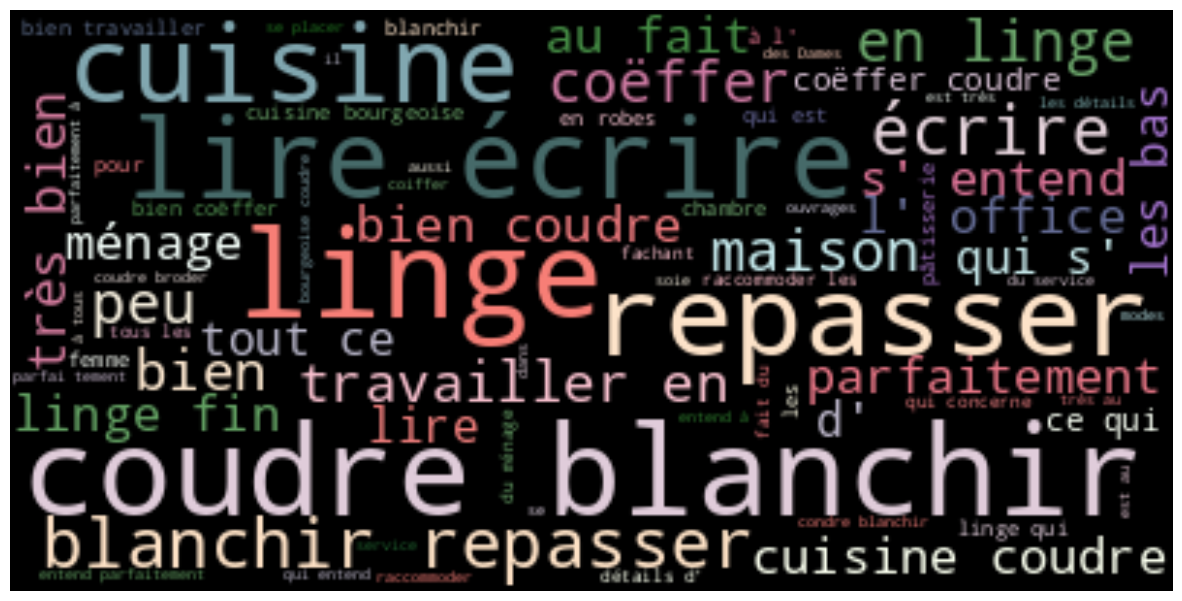
\includegraphics[width=6cm]{wordcloud_comp_F.png}
	\end{subfigure}
	\begin{subfigure}[b]{0.4\textwidth}
		\centering
		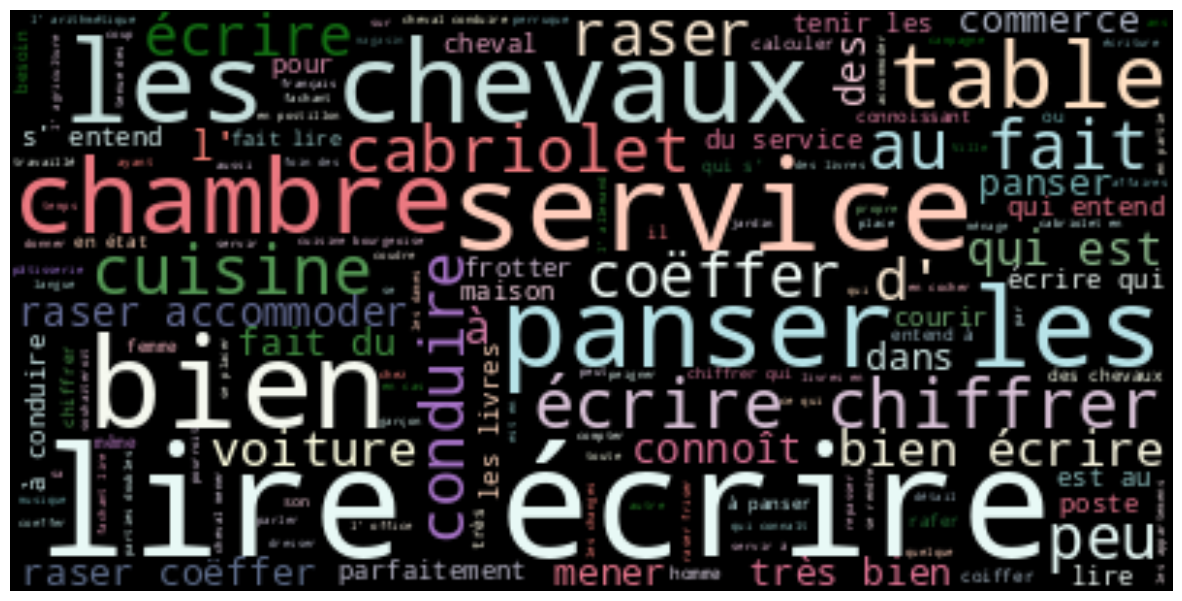
\includegraphics[width=6cm]{wordcloud_comp_H.png}
	\end{subfigure}
	\caption{Nuage de mots des compétences dans les annonces écrites par des femmes (gauche) et par des hommes (droite)}
\end{figure}


\subsection{Des compétences féminines confinées à l'intérieur du foyer}

Comme on peut l'observer à l'aide du nuage de mots ci-dessus et du tableau de fréquences suivant, les compétences féminines ont principalement trait à deux pôles d'activités: le soin du linge et la cuisine. Des activités non seulement peu qualifiées, mais surtout localisées à l'intérieur même du foyer (à l'exception notable du blanchissage, qui peut se faire à l'intérieur ou, plus couramment à Paris, sur les rives de la Seine et de la Bièvre), et qui se caractérisent par leur multiplicité: "savoir tout ce qui a trait au linge" signifie non seulement savoir le laver, le raccommoder, le repasser, mais également savoir fabriquer des pièces à la main. 

\begin{table}[ht]
	\centering
	\begin{tabular}{|l|c|}
		\multicolumn{1}{|c|}{\textbf{Mot}} & \textbf{Occurrences} \\ \hline
		blanchir                         & 203                  \\
		coudre                           & 197                  \\
		linge                            & 177                  \\
		repasser                         & 152                  \\
		écrire                           & 135                  \\
		cuisine                          & 131                  \\
		lire                             & 102                  \\
		parfaitement                     & 55                   \\
		coiffer                          & 52                   \\
		travailler                       & 48                  
	\end{tabular}
	\caption{Dix mots les plus fréquents parmi les compétences d'annonces de femmes}
\end{table}

L'omniprésence du linge parmi les compétences féminines est proportionnelle à son importance croissante dans l'économie domestique du XVIIIè siècle\footcites{rocheInventionLingeAu1986}, et au temps nécessaire à son soin durant l'ère pré-industrielle. Avoir du personnel compétent en la matière est alors essentiel: porter des chemises jaunies, servir à manger sur une nappe tâchée sont autant de fautes qui mettent en exergue la place du linge dans la "hiérarchie du paraître\footcites[p.236]{rocheInventionLingeAu1986}". À ces motifs de distinction sociale s'ajoutent également au cours du XVIIIè siècle des raisons hygiénistes\footcites{ungererValeursUrbainesPropre1986}, qui exacerbent encore l'importance d'un linge bien blanchi.

L'association des femmes à cette activité découle en grande partie de leur association plus générale au textile. La couture, notamment, devient une occupation intégralement féminine au cours des XVIIè-XVIIIè siècles, caractérisés par la perte de la main-mise de la communauté des tailleurs sur ce secteur d'activités\footcites{crowstonFabricatingWomenSeamstresses2001}{crowstonEngenderingGuildsSeamstresses2000}. Au moins jusqu'à la fin du siècle\footcites{moreraBlanchisseusesPropreBlanchisseurs2018}, le lavage du linge et les savoir-faire qui lui sont liés sont également l'apanage de femmes, qu'elles soient domestiques ou blanchisseuses spécialisées.

Au-delà des aptitudes fondamentales que constituent la couture, le blanchissage et le repassage, certaines annonces mentionnent également des compétences textiles plus rares et particulières, qui les distinguent autant qu'elles les destinent à un certain type d'employeurs: l'évocation du lavage des bas (56 occurrences), de la broderie (62) ou de certaines matières précieuses comme la soie (43) ou la dentelle (17) correspond à certains besoins et certaines demandes spécifiques des employeurs les plus fortunés.


La cuisine, quant à elle, constitue une autre activité culturellement associée à la féminité. Au XVIIIè siècle, avec l'avènement d'un savoir-vivre "à la française", qui repose en grande partie sur la gastronomie, le métier de cuisinier se masculinise, notamment dans les maisons bourgeoises et nobles où il est en vogue d'employer un "chef de haute cuisine" qui se distingue fortement du reste de la domesticité, par sa rémunération comme par son statut\footcites[p.25-35]{sabattierFigaroSonMaitre1984}. Mais dans le foyer ordinaire, la cuisine dite "de ménage" reste majoritairement une affaire de femmes\footcites{drouardChapitrePremierCuisiniers2016}. 

Comme dans le cas du linge, si sa mention dans l'annonce représente surtout un moyen de signifier la pluricompétence d'une domestique (savoir blanchir, coudre et cuisiner signale, dans la domesticité modeste, une capacité à tenir une maison seule ou presque), elle peut également prendre une valeur distinctive dès lors qu'elle s'accompagne d'adverbes ou d'adjectifs mélioratifs (faire une "très bonne cuisine" ou une cuisine "bourgeoise") voire même de spécialisations culinaires. La pâtisserie, notamment, est le vingtième talent le plus fréquent dans ce corpus féminin. 

Ainsi, dans le cas de la domesticité féminine, c'est la multiplicité des compétences et la pluri-activité qui priment: si la cuisine ou le soin du linge sont bien identifiés comme activités spécifiquement destinées aux femmes, c'est surtout l'agrégation des compétences qui valorise leur candidature, et qui les rattache au service peu qualifié, de petite maison. Les annonces de femmes sont ainsi en moyenne plus longue que les annonces d'hommes (76 mots en moyenne contre 70) et contiennent aussi plutôt plus de verbes de compétences (3,5 verbes en moyenne contre 3,1 pour les hommes). Mais c'est surtout la présence de certaines expressions englobantes, cherchant à signifier une maîtrise complète des arts de la maison, qui caractérisent les annonces de femmes, alors qu'elles sont pratiquement absentes chez leurs homologues masculins: une annonce sur cinq contient des expressions semblables à "capable de rendre tous les services pour l'intérieur d'un ménage", "très au fait de la tenue d'une maison", "sachant [...] tout ce qui concerne la manutention d'un ménage".

\subsection{Des compétences masculines tournées vers l'extérieur de la maison et le service du maître}

Les annonces masculines relèvent d'un tout autre registre. Les compétences qu'elles renferment sont, quant à elles, principalement liées au service particulier d'un maître ou à des activités de plein air et de transport. 

Les références au service personnel ont la particularité de beaucoup se référer à la pilosité: "coiffer" et "raser" sont parmi les termes les plus communs, soulignant à la fois le rôle central du valet ou du domestique particulier dans l'apparence de son maître, et l'importance d'être bien rasé durant un siècle où, pour une fraction de la population, la barbe est synonyme de déchéance sociale ou de barbarie \footcites{auzepyHistoirePoil2017}. Certaines annonces mentionnent même savoir "coiffer femmes et hommes"; si la femme de chambre est souvent chargée de coiffer sa maîtresse au quotidien, le métier ou l'art de coiffer est globalement masculin. 

Le second ensemble de compétences masculines se rapporte aux activités d'extérieur, et notamment au transport du maître: savoir conduire un cabriolet ou une voiture, s'occuper des attelages. Là encore, la fonction pratique du domestique va de pair avec une dimension ostentatoire; l'homme domestique est celui qui sort en ville et accompagne son maître partout où il va. L'importance du cheval dans les annonces est proportionnelle à l'importance de celui-ci dans la ville: élément de distinction par rapport au peuple qui va à pied, il devient progressivement indispensable aux déplacements et donc à la vie sociale des maîtres sous l'Ancien Régime\footcites{rocheCultureEquestreOccidentale2008}. 


\begin{table}[ht]
	\centering
	\begin{tabular}{|l|c|}
		\multicolumn{1}{|c|}{\textbf{Mot}} & \textbf{Occurrences} \\ \hline
		écrire                           & 342                  \\
		lire                             & 218                  \\
		chevaux                          & 150                  \\
		service                          & 136                  \\
		panser                           & 134                  \\
		raser                            & 128                  \\
		chiffrer                         & 92                   \\
		chambre                          & 76                   \\
		conduire                         & 75                   \\
		cuisine                          & 68                  
	\end{tabular}
	\caption{Dix mots les plus fréquents parmi les compétences d'annonces d'hommes}

\end{table}


Ainsi, la division sexuée des tâches domestiques dans les annonces reproduit la division spatiale des sexes dans l'espace social, rendue visible par l'énonciation des compétences: les femmes valorisent un savoir-faire qui s'exerce à l'intérieur du foyer, dans le cadre d'activités qui leur sont culturellement dédiées (couture, cuisine, ménage) et par ailleurs peu qualifiées et dévalorisées. Les hommes, à l'inverse, font état de compétences plus spécifiques et plus gratifiantes dans l'imaginaire et la hiérarchie de la domesticité, sans être forcément beaucoup plus qualifiées: le service spécifique d'un maître, qui implique de pénétrer dans sa chambre et donc dans son intimité, ainsi que le soin de son transport et de ses déplacements, qui induit une présence à l'extérieur, une visibilité sociale et un accompagnement de chaque instant. 

Certains indices, minoritaires dans les annonces mais tout de même présents, permettent néanmoins de relativiser ce premier constat d'une division forte, voire étanche, des sexes au travail: certaines annonces d'hommes (68 sur 607, soit un peu plus d'une sur dix) font ainsi référence à la cuisine. Mais cette mention se fait le plus souvent au milieu de nombreuses autres compétences, et en précisant qu'il s'agit d'une compétence additionnelle mais qui ne constitue pas le cœur du travail du domestique: ainsi, dans une annonce masculine mentionnant la cuisine sur quatre, le demandeur précise faire seulement "un peu de cuisine" ou faire la cuisine "en cas de besoin", insistant encore sur le caractère de compétence "d'appoint" de ce savoir-faire pour les hommes. 


\subsection{"Sachant l'anglais, l'allemand et un peu d'italien": une domesticité qualifiée et intellectuelle surreprésentée dans les annonces}

Enfin, un dernier sous-ensemble du corpus, minoritaire mais tout de même significatif, concerne les compétences qui ne sont pas manuelles mais relèvent au contraire de capacités intellectuelles, qui mobilisent l'écriture ou un capital culturel. Parmi celles-ci, beaucoup concernent l'enseignement ou la connaissance d'une ou plusieurs langues; elles sont principalement écrites par des hommes, plutôt plus âgés que la moyenne des demandeurs.

J'ai déjà évoqué plus tôt la présence massive des références au triptyque "lire, écrire, chiffrer", sans préciser cependant que celui-ci est réparti très inégalement selon le sexe dans les petites annonces: 54\% des annonces d'hommes évoquent le fait de savoir lire, contre 36\% annonces de femmes. 59\% des annonces masculines mentionnent l'écriture, contre 28\% des annonces féminines; enfin, 13\% des hommes font état d'une compétence liée aux chiffres, contre 2\% des femmes. Ainsi, ces compétences sont majoritairement présentes chez les hommes: on attend d'un domestique masculin non seulement qu'il accomplisse ses tâches et travaux manuels, mais également qu'il puisse ponctuellement ou régulièrement aider son maître dans ses affaires professionnelles ou sa sociabilité, en écrivant une lettre, en faisant ses comptes, ... 

Cette "masculinité" des compétences intellectuelles s'applique également à des talents plus spécialisés. La connaissance ou l'enseignement d'une ou plusieurs langues, notamment, dont l'importance dans les annonces a déjà été attestée par Ulrike Krampl\footcites{kramplTravaillerAvecLangues2019}, se retrouve dans ce corpus: 106 domestiques disent pouvoir "enseigner" (dont 47 hommes, 12 femmes, et 47 domestiques dont le sexe n'a pas pu être déterminé). 93 annonces mentionnent les langues, qu'il s'agisse de l'enseigner ou de savoir la parler: 54 hommes, neuf femmes, 30 domestiques indéterminés. Parmi ces langues, on trouve en premier lieu l'allemand (mentionné par 50 demandeurs, dont 28 hommes), puis l'italien (33 mentions, dont 25 par des hommes), l'anglais (26 occurrences) et l'espagnol (4 occurrences).

Mais les langues ne sont pas les seuls enseignements présents dans les annonces: la géographie (28 occurrences) et l'histoire (21 occurrences) sont également représentées, ainsi que la musique, qui a la particularité d'être plutôt un art enseigné par des femmes (24 mentions, dont 8 par des femmes et 4 par des hommes). Ces disciplines, intellectuelles et artistiques, semblent signaler que les domestiques qui les mentionnent cherchent une place de précepteur ou de gouvernante, dont l'emploi dans les grandes maisons croit au XVIIIè siècle avec l'importance renouvelée accordée à l'éducation \footcites{sabattierChapitreIntimiteConstante1984}.

Plus rarement, les enseignements mentionnés sont manuels, liés à la maîtrise de la couture ou à la tenue de la maison, enseignés par des femmes et destinés plutôt aux jeunes filles: "Une Demoiselle d'un âge mûr, qui a reçu une éducation soignée, et qui appartient à une famille honnête, désirerait se placer en qualité de Personne de compagnie, à la ville ou à la campagne; elle est au fait des soins d'un ménage, et en état d'enseigner la couture, la broderie, et autres ouvrages\footnote{\textit{Affiches de Lyon}, 20 avril 1803"; "Une Citoyenne âgée de quarante-cinq ans, désirerait se placer dans quelque maison pour l'éducation de jeunes personnes; elle leur enseignerait la lecture; l'écriture, la couture, la broderie, à raccommoder dentelle\footnote{\textit{Affiches de Lyon}, 16 septembre 1795}". Même chez une domesticité plus qualifiée, la différenciation des sexes par espace et champ d'expertise est reproduite. 


\bigskip

Ainsi, l'étude des compétences et des savoir-faire dans les annonces d'emploi informe indirectement sur la division sociale et sexuée du travail domestique. Les femmes mettent en avant des compétences multiples, de servantes ou de bonnes à tout faire: cuisine et linge, tandis que celles des hommes sont plus spécialisées, et les rapprochent plutôt de l'état de valet. Néanmoins, la présence, voire la surreprésentation, dans les annonces, d'une domesticité plus qualifiée, liée à l'enseignement, au préceptorat ou au secrétariat particulier, semble indiquer une spécificité de la domesticité d'annonces par rapport à la population domestique générale: "loin de se réduire à un miroir de l’état du marché, le journal circonscrit un segment spécifique, davantage masculin et souvent qualifié du marché du travail\footcites{kramplPresseAnnoncesParisienne2020}". 



\chapter{"D'un extérieur agréable, aux mœurs honnêtes": la mise en valeur de soi dans les annonces}

La ou le domestique du XVIIIè siècle n'a pas uniquement une fonction pratique d'accomplissement de tâches trop physiques, trop basses ou trop chronophages pour ses maîtres. Il ou elle est également membre d'une maison, ainsi que le discours paternaliste des moralistes et des observateurs sociaux s'efforce de le rappeler au XVIIIè siècle\footcites{sabattierChapitreEnseigneSon1984}. À ce titre, s'ajoute à sa charge laborieuse une charge de représentation de ses maîtres et de sa maison. Cette charge est d'autant plus importante lorsque les domestiques sont voués à se montrer, comme le sont les domestiques de la livrée, valets et laquais notamment. 

En sus de devoir répondre à certains critères physiques, les domestiques doivent également surmonter les préjugés moraux qui les accablent à l'époque moderne: membres d'une classe dangereuse, ils et elles sont présentées par les traités de police et les manuels de savoir-vivre comme prédisposés au vol, au mensonge, à l'injure, à l'escroquerie et aux mauvaises mœurs\footcites{sabattierChapitreOpinionDefavorable1984}. 

Ainsi, les annonces ne sont pas seulement un résumé d'un parcours de vie ou une énumération méthodique de compétences, mais également un espace où la mise en valeur de soi est essentielle, pour distinguer sa candidature et montrer sa conformité aux attendus physiques et moraux de la domesticité. 


\section{Méthode}

Pour s'intéresser aux descriptifs et aux qualificatifs personnels dans les annonces, j'ai tout d'abord employé une première méthode exploratoire dédiée à l'extraction des adjectifs qualificatifs du corpus avec la librairie Spacy, qui m'a permis de réaliser le nuage de mots suivant. Néanmoins, cette méthode simple présente de nombreuses limites, la plus importante étant qu'elle ne permet pas de discriminer entre les adjectifs se référant au domestique qui rédige l'annonce, et les adjectifs se référant à d'autres noms ("une cuisine bourgeoise", "une maison honnête"). De plus, elle relève également des adjectifs qui ne sont pas des qualités mais simplement des descripteurs ("âgé", "veuve").

\begin{figure}[h]
	\centering
	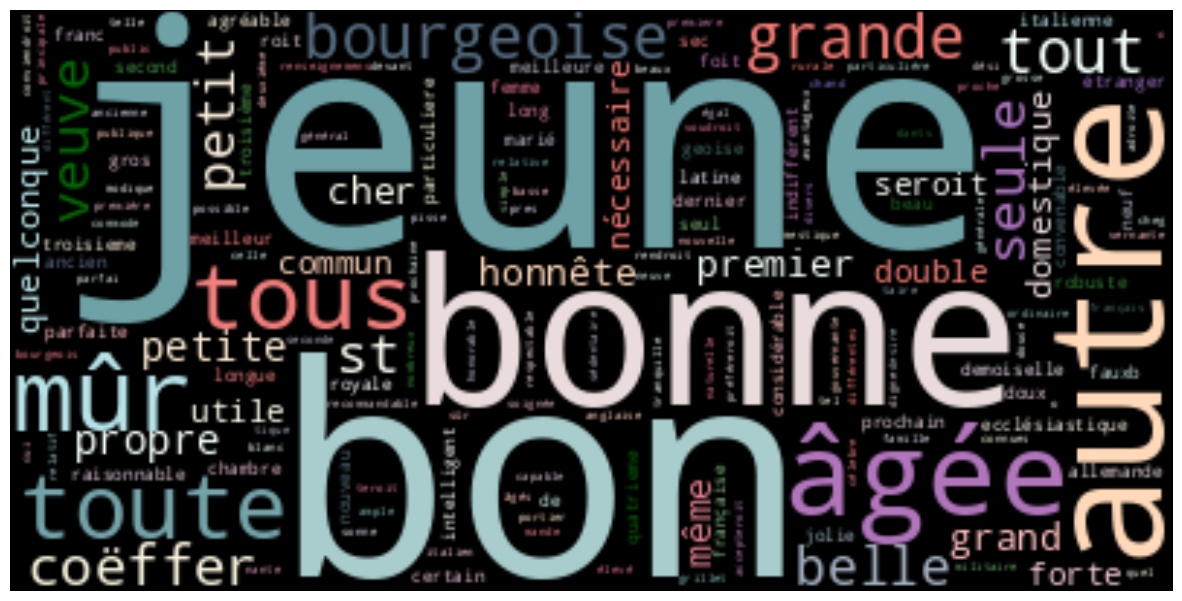
\includegraphics[width=12cm]{wordcloud_qualites_adj.png}
	\caption{Nuage de mots des adjectifs dans le corpus}
\end{figure}


Comme dans le cas des compétences, la deuxième méthode envisagée a alors consisté en l'entraînement d'un modèle de \textit{span categorization} avec spacy, toujours sur la base d'environ 500 annonces annotées, mais dont les annotations étaient cette fois dédiées aux qualités. Cette méthode s'est également révélée décevante: j'ai observé en annotant que les annonces mentionnant des qualités sont peu nombreuses (parmi les 500 que j'ai annotées, moins d'une sur dix en contient). L'entraînement du modèle a donc généré des scores de performance très faibles, voire nuls.

Face à l'échec de ces deux premières méthodes, mais maintenant forte d'une meilleure connaissance du corpus à la suite de l'annotation, j'ai donc fini par avoir recours à une méthode beaucoup plus artisanale, basée sur un mélange d'expressions régulières, de recherche de mots-clés et d'extraction d'adjectifs (à l'exception de "âgé", présent dans beaucoup d'annonces mais qui ne m'intéressent pas ici). J'ai en outre décidé de cantonner cette méthode aux dix premiers mots de chaque texte du corpus, ayant observé que les qualités que je souhaitais extraire étaient souvent placées au début de l'annonce. 

À l'aide de la fonction ci-dessous, je suis finalement parvenue à extraire des qualités pour 3096 annonces, dont on peut avoir un aperçu grâce au nuage de mot suivant. Si les adjectifs déjà présents avec la première méthode restent très visibles (jeune, bon, bonne), d'autres éléments apparaissent néanmoins: des qualificatifs physiques (jolie, agréable, ...) comme moraux ou intellectuels (recommandable, bien élevé, intelligent...). Le format du nuage de mots n'est cependant pas très utile pour restituer la présence dans le corpus d'expressions et de groupes de mots, pourtant très employés dans les annonces.

\begin{lstlisting}[language=Python,caption=Fonction destinée à extraire les qualités des annonces]
def extraire_qualites(annonce):
	qualites=[]

	# Extraire les adjectifs
	doc = nlp(annonce) 
	for token in doc:
		if token.pos_=="ADJ":
			qualites.append(token.text)
	
	qual_a_retirer=["age", "agee"]
	
	# Regex qui permet d'extraire les expressions descriptives du type "d'un beau physique", "aux moeurs honnetes"
	regex=", ?((?:d'|de |dont |au |aux )\w+'? ?\w+ (?:\w+)? (?:\w+)?),"
	qualites_regex=re.findall(regex, annonce, re.UNICODE)
	for i in qualites_regex:
		qualites.append(i)

	return " ".join(i for i in qualites if i not in qual_a_retirer)
\end{lstlisting}


\begin{figure}[ht]
	\centering
	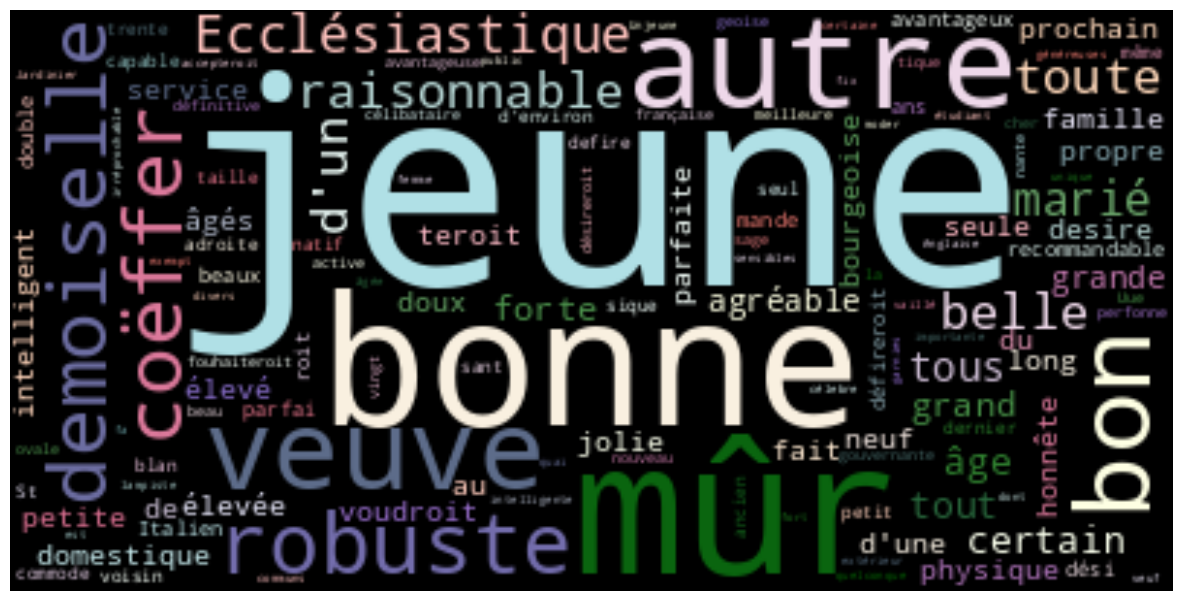
\includegraphics[width=12cm]{wordcloud_qualites.png}
	\caption{Nuage de mots des qualités dans le corpus}
\end{figure}


\section{La mise en valeur physique et intellectuelle, apanage d'une domesticité vouée à se montrer}

Un examen plus approfondi des qualités dans les annonces montre que la plupart d'entre elles se réfèrent au physique du ou de la domestique. Hormis l'adjectif "jeune", les termes les plus fréquents parmi les qualités extraites comprennent entre autres "grand" (348 occurrences), "fort" (376 occurrences), "belle" (159 occurrences), "agréable" (49 occurrences), "intelligent" (47 occurrences), "doux" (36 occurrences).

Les qualités relatives à la force et à la taille sont très majoritairement masculins: plus de trois occurrences de l'adjectif "robuste" sur quatre se trouvent dans des annonces d'hommes. Il en est de même pour l'expression "d'une belle taille" et l'adjectif "grand". La taille a une importance toute particulière dans l'embauche d'un domestique, notamment d'un valet ou d'un laquais, qui doit faire bonne figure auprès de son maître et chez qui une grande taille et une belle posture sont des indicateurs de bonne santé autant que de dignité\footcites{sabattierChapitreConditionDomestique1984}. L'intelligence figure également en bonne place parmi les qualités les plus mentionnées; encore une fois, elle est surtout masculine (65\% des annonces). 


\section{La mise en valeur morale, une qualité surtout féminine}

Un second ensemble des qualités extraites des annonces se rapporte cette fois plutôt à la moralité et à l'honnêteté des domestiques. Se présenter comme "honnête" (261 occurrences dans le corpus), ayant de "bonnes mœurs", une "bonne moralité" (254 occurrences), issue d'une bonne famille (93 occurrences) ou faisant preuve de "probité" (86 occurrences) sont autant de moyens de contrecarrer la mauvaise réputation imputée aux travailleuses et travailleurs de la domesticité. Mais ces qualités morales sont cette fois surtout l'apanage des femmes: 21\% des annonces féminines mentionnent l'honnêteté ou la probité, contre 13\% de celles des hommes. 

Aux hommes la force, aux femmes l'intégrité? Si cette distinction reproduit les attendus culturels associés aux deux sexes, la raison de sa présence parmi les annonces est peut-être plutôt à chercher du côté des conditions de travail des domestiques hommes et femmes, et donc aux préjugés et aux attendus qui leur sont associés. On l'a déjà vu, les (jeunes) hommes, qui cherchent à entrer au service d'un maître en tant que domestique particulier, une fonction qui implique de beaucoup se montrer, savent que leur physique est important sinon central, et cherchent donc à se mettre en valeur en conséquence. Les femmes, au contraire, sont chargées de tâches au sein de la maison, en ayant souvent accès au linge, à l'argenterie et à d'autres items personnels qui peuvent faire l'objet de convoitises et donc de vols de la part des domestiques. De plus, leur sexualité et leurs relations font l'objet d'une surveillance plus importante que leurs homologues masculins. On peut supposer que face à ces accusations et à cette méfiance, se présenter comme honnête (qualité renforcée ensuite par la référence à de "bons répondants") encourage voire conditionne l'embauche.


\bigskip


Les annonces d'emploi font ainsi l'objet de mises en récit et de phénomènes de publicité de soi et de son travail qui ne sont pas sans rappeler les annonces matrimoniales de la même période \footcites{jonesPersonalsPoliticsCourting2001}. La tendance est à la présentation méliorative de soi-même, de son physique comme de sa moralité, en conformité avec les normes qui entourent le travail ancillaire au XVIIIè siècle. 

Mais parfois, des  annonces sous forme de "récits de vie" semble font plutôt faire appel au registre pathétique:  "Une jeune veuve, d'un physique agréable, ayant reçu de l'éducation, appartenant à une honnête famille, ayant éprouvé de très-grands malheurs, voudroit trouver une PLACE auprès d'une personne seule pour prendre soin de son ménage, ou pour tenir un comptoir\footnote{\textit{Affiches de Paris}, 27 février 1804}"; "Une veuve âgée de 30 ans, sans suite, d'un caractère gai et doux, et d'une bonne famille, que des malheurs forcent à chercher une PLACE, desire en trouver une quelconque\footnote{\textit{Affiches de Paris}, 6 mars 1804}". Si la recherche d'emploi domestique à l'époque moderne ressemble par beaucoup d'aspects à celle d'aujourd'hui, basée sur la valorisation personnelle, d'autres éléments des annonces rappellent la dimension charitable de la domesticité au XVIIIè siècle: dans la loi comme dans les traités religieux, prendre un domestique, c'est également porter assistance aux plus démunis, en fournissant gages et logis\footcites{sabattierChapitreMaitrePere1984}. Les journaux d'annonces eux-mêmes, à leurs débuts, sont pensés comme des outils de gestion des populations indigentes, et les Bureaux d'adresses, nés du traité \textit{Sur la condition des pauvres} de Théophraste Renaudot, visent à devenir des alternatives à l'Église dans le traitement de la pauvreté. Une dimension qui transparaît également à travers l'absence presque totale de revendications (salariales ou autres) dans les annonces: dans le contexte de crise de l'emploi qui touche les grandes villes française de la seconde moitié du XVIIIè siècle, le marché de l'emploi domestique est à l'avantage des employeurs.

\chapter{Demander sans quémander: des modalités d'emploi absentes des annonces}

La mise en valeur de soi et de son travail se fait souvent aux dépends d'autres éléments dans l'annonce: les conditions matérielles d'emploi. Comment expliquer cette absence: économie de l'espace par le journal, information jugée dérisoire car tacite? 


\section{Méthode}

Les "modalités d'emploi" que je cherche à relever dans les annonces se divisent en deux ensembles. D'un côté, l'emploi ou le métier recherché; de l'autre, les conditions concrètes de travail, qui comprennent notamment les gages demandés. 

Pour ce qui est de l'emploi recherché, j'ai annoté le corpus puis entraîné un modèle de \textit{span categorization } pour reconnaître les noms de professions, de métiers et d'occupations parmi les annonces. Cette méthode a permis d'extraire une mention d'emploi dans 1506 annonces. 

Pour les gages et les conditions d'emploi plus générales, j'ai estimé que le corpus était assez homogène pour que l'analyse puisse se faire à l'aide de mots-clés. 

\section{"Cherche une place de...". Une revendication commune: l'emploi recherché}


Si l'identité professionnelle n'a pas encore sous l'Ancien Régime la valeur ni l'uniformité qu'elle prendra au XIXè puis au XXè siècle, cela n'empêche pas les domestiques en recherche d'emploi de privilégier certaines places, en raison de leur formation ou de leurs compétences. Si la majorité des domestiques travaille dans des petits foyers, où leur labeur est peu spécialisé, d'autres se trouvent au contraire insérés dans des hiérarchies ancillaires complexes, où femmes-de-chambres, valets, cochers et cuisiniers n'ont ni les mêmes tâches, ni les mêmes rémunérations, ni le même rapport à leurs maîtres. 

\begin{figure}[ht]
	\centering
	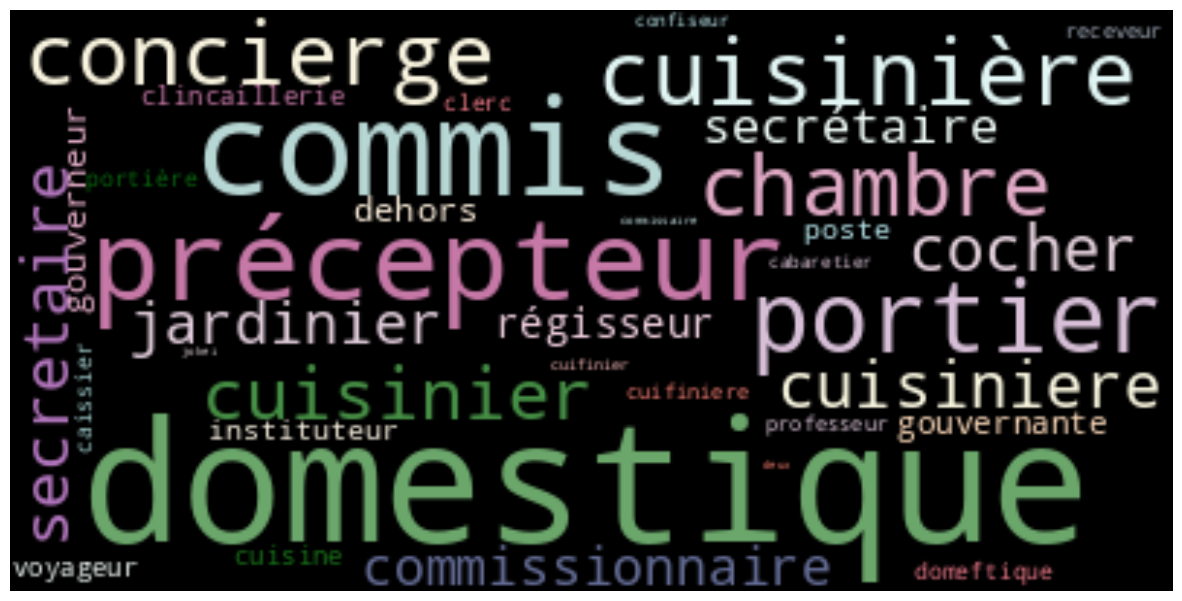
\includegraphics[width=12cm]{wordcloud_emploi.png}
	\caption{Nuage de mots des noms d'emplois dans le corpus}
\end{figure}

Les annonces reflètent cette réalité de la domesticité: si plus de deux annonces sur trois ne mentionnent pas d'emploi précis, ou alors en utilisant un qualificatif très général ("domestique"), le reste se caractérisent au contraire par la mention d'une grande diversité de rôles et de fonctions différentes: de la domesticité de confiance (secrétaire, régisseur, commissionnaire) à la domesticité chargée de l'éducation (gouvernante, gouverneur, précepteur), en passant par celle chargée d'espaces très circonscrits de la maison (jardinier, portier, cuisinier et cuisinière). 

De la même façon que les compétences ou les qualités que j'ai déjà mentionnées, les emplois sont eux aussi sexués: on observe une moins grande diversité des rôles mentionnés par les femmes, qui cherchent pour la plupart à se placer en tant que femme de chambre, cuisinière ou gouvernante, que pour les hommes, où la pluralité des conditions provient surtout des emplois domestiques plus qualifiés, souvent très spécialisés (secrétaire, instituteur, précepteur...).


\begin{table}[ht]
	\centering
	\begin{tabular}{lc}
		\hline
		\multicolumn{1}{c}{\textbf{Emploi}} & \textbf{Occurrences} \\ \hline
		domestique                          & 315                  \\
		commis                              & 153                  \\
		précepteur                          & 128                  \\
		cuisinière                          & 124                  \\
		valet                               & 86                   \\
		femme de chambre                    & 69                   \\
		portier                             & 68                   \\
		secrétaire                          & 51                   \\
		concierge                           & 45                   \\
		cuisinier                           & 45                   \\
		jardinier                           & 33                   \\
		cocher                              & 25                   \\
		commissionnaire                     & 22                   \\
		régisseur                           & 13                   \\
		gouvernante                         & 13                   \\
		gouverneur                          & 12                  \\ \hline
	\end{tabular}
	\caption{Emplois les plus fréquents dans le corpus (plus de dix occurrences)}
\end{table}


\begin{figure}[ht]
	\centering
	\begin{subfigure}[b]{0.4\textwidth}
		\centering
		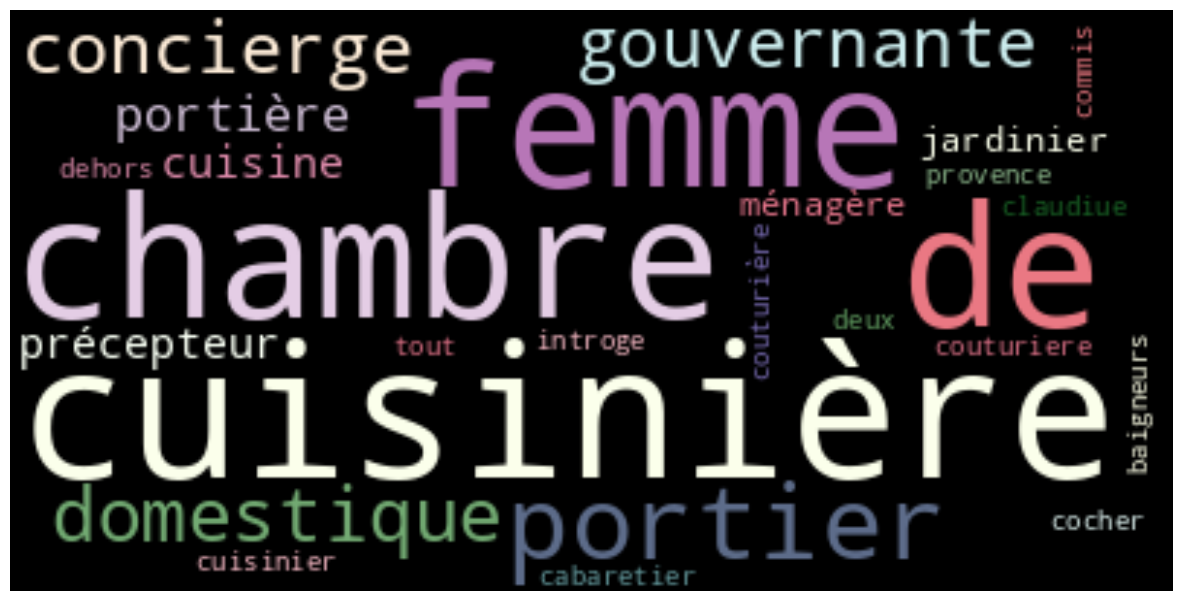
\includegraphics[width=6cm]{wordcloud_emploi_F.png}
	\end{subfigure}
	\begin{subfigure}[b]{0.4\textwidth}
		\centering
		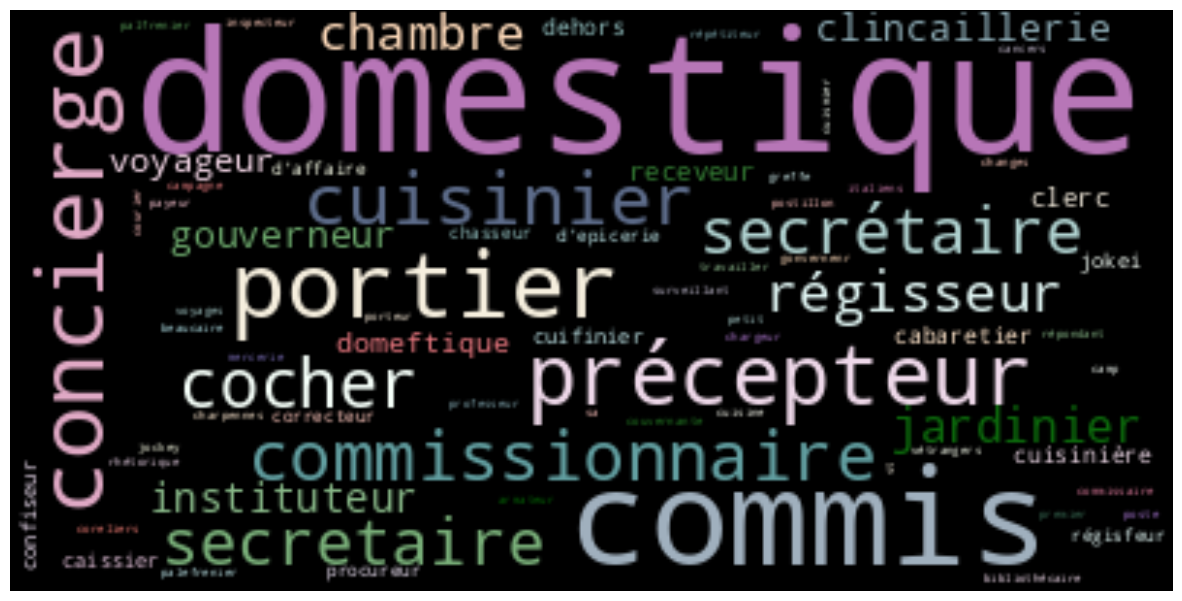
\includegraphics[width=6cm]{wordcloud_emploi_H.png}
	\end{subfigure}
	\caption{Nuage de mots des compétences dans les annonces écrites par des femmes (gauche) et par des hommes (droite)}
\end{figure}


Enfin, l'étude des \textit{Affiches} est également l'occasion d'observer l'apparition d'activités moins communes, concomittantes de certaines transformations de l'espace urbain, comme dans cette annonce parisienne en date du 18 mars 1804: "Un homme et sa femme, sans enfans, ayant travaillé dans les bains les plus en réputations de Paris, possédant toutes les connaissances requises pour ce genre de travail, entr'autres celle des bains épilatoires des douches et de vapeur et de propretés en se baignans ou sans se baigner, desirent se PLACER comme baigneurs, soit à Paris ou dans les départemens; à Paris ils leur seroit indifférent de se placer séparément. S'adresser par écrit, au portier de ce Journal\footnote{\textit{Affiches de Paris}, 18 mars 1804}."


\section{L'omission des gages et des conditions de travail : stratégie ou nécessité? }

Face à cette présence minoritaire mais régulière des noms de métiers et des spécialisations domestiques dans les annonces, l'absence de revendications de rémunérations ou de conditions de travail apparaît encore plus flagrante.

Gages et appointements sont presque inexistants dans le corpus. Seules 48 annonces mentionnent d'une façon ou d'une autre une rémunération: parmi elles, 41 disent "se contenter d'un appointement modique" (parfois limité à la table ou au logis) voire ne pas exiger de gages du tout (parfois pour une période donnée, parfois avec des justifications assez absurdes: "quoi-que ses talents méritent des appointements, il n'en exigera point\footnote{\textit{Affiche de Lyon}, 11 juin 1772.}", parfois en précisant avoir un autre revenu, le plus souvent une rente), trois ont des revendications précises, parfois liées à des qualifications ou des spécialisations domestiques ("pas moins de 200 francs\footnote{\textit{Affiches de Paris}, 19 mars 1804.}", "ne se déplacera pas qu'on ne lui donne un avantage et cent écus ou au moins deux cents cinquantes livres de gages par an\footnote{\textit{Affiches de Lyon}, 30 août 1769.}", "deux à trois cents livres d'appointement par an\footnote{\textit{Affiches de Lyon}, 14 octobre 1767.}"), et quatre sont des offres d'emploi.
 
En dehors des gages, les seules revendications de la part des domestiques consistent généralement à demander à se placer "dans quelque bonne maison" (255 annonces), ou auprès de personnes spécifiques: femmes ou hommes seuls, ou au contraire dans des maisons avec de jeunes enfants. Les demandes liées à une envie de voyager (252 annonces) ou de vivre à la campagne sont également relativement nombreuses, et témoignent de l'espace de liberté et d'ouverture des possibles que représente le journal de petites annonces, ainsi que l'a déjà signalé Ulrike Krampl\footcites{kramplAdresserClercHuissier2017}. 

Sans comparaison avec d'autres périodicités, il est difficile de dire si cette absence des conditions de travail est commune dans les annonces, les gages étant discutés de vive voix, ou si elle résulte d'un contexte économique difficile pour les domestiques, qui se voient obligés d'accepter les gages et les circonstances proposées par les employeurs. 

